\chapter{Simple BSP-based model to predict CUDA kernels}\label{chap:BSPmodel}
Models are useful to represent abstractions of software and hardware processes. The Bulk Synchronous Parallel (BSP) is a bridging model for parallel computation that allows algorithmic analysis of programs on parallel computers using performance modeling. The main idea of the BSP model is the treatment of communication and computation as abstractions of a parallel system.

In this chapter, we present a simple and intuitive BSP-based model for predicting the CUDA application execution times on GPUs. The model is based on the number of computations and memory accesses of the GPU, with additional information from profiling. Scalability, divergence, effect of optimizations and differences of architectures are adjusted by a single parameter.

The structure of this chapter is organized as follow,  in Section~\ref{sec:BackgroundModel} we mention the most important parallel models of the literature, in Section \ref{sec:proposeModel}, we describe the propose parallel BSP-based model to predict execution time of GPU applications, in Section~\ref{sec:methodModel} we describe the methodology and the use cases, in Section~\ref{sec:resultModel} we show some experimental results and  finally in Section~\ref{sec:relatedModel} we show the main relate works of this model.







\section{Review of Parallel Computational Models}
\label{sec:BackgroundModel}

The basic computer architecture is known as von Neummann architecture or von Neumman model. This model has the following components: a memory; an arithmetic-logic unit (ALU); a central processing unit (CPU), composed of several registers; and a control unit. New technologies and computational models began to be developed simultaneously with the evolution of the von Neumann model. 

In 1972, Michael Flynn proposed a classification of parallel computing architectures. This classification distinguishes the number of instructions and the number of data that can be computed in parallel~\citep{flynn1996parallel}. This classification is presented in the Table \ref{tab:taxFlynn}.

\begin{table}[htpb]
\begin{center}
\begin{tabular}{|r|c|c|}
\hline
& \bf Single Instruction & \bf Multiple Instruction\\\hline 
\bf Single Data & SISD & MISD \\\hline 
\bf Multiple Data & SIMD & MIMD \\\hline 
\end{tabular}
\end{center}
\caption{Classification of parallel architectures proposed by Michael Flynn (1972).} 
\label{tab:taxFlynn}
\end{table}

We can illustrate the table above as follows. A von Neumann model machine that has only one processing core fits the SISD (Single Instruction; Single Data) classification; a machine with multiple processing cores can be classified as MIMD; GPUs are classified on the SIMD architecture, where each thread takes index to perform vector computations, for this the programming model of CUDA is named SIMT (Single Instruction; Multiple Threads).

Parallel computing models have been an active research topic since the development of modern computers~\citep{Gibbons1983:QRQW,Juurlink:1998,Skillicorn:1998:MLP}; their main goal is to provide a standard way of describing and evaluating the performance of parallel applications. For the success of a parallel computing model, it is paramount to also consider the characteristics of the underlying architecture of the hardware being used.


Mathematical models are simplified abstraction of a real situation. A important area of the computer science is related with the analysis, design and development of algoritmh that are implemented in real machines. A first and general example is the RAM model (Random-Access Memory). This model is an abstraction of a classic computer with a single processor. More and not a few models were created based on the RAM model.

In computing, granularity is associated with the amount of computation in relation to communication, that is, the ratio of computation to the amount of communication. Parallelism of fine granularity means relatively small amounts of computational work are done between communication events
Low computation to communication ratio. Coarse and Bulk granularity is the opposite: data transfers are less frequent, and present large amounts of computation. Parallelism of coarse or Bulk granularity means relatively large amounts of computational work are done between communication events, high computation to communication ratio. The finer granularity have greater potential for parallelism and consequently the increase in speed, but the overhead costs of synchronization and communication are expensive in terms of latency.

The main objective of a parallel computing model is to provide a set of parameters to be considered in the implementation of a parallel algorithm. These parameters can be used to simulate the behavior of applications that will run on different parallel platforms. To facilitate the programming and simulation of these applications, models with specific properties to parallel programming problems have been created~\citep{Skillicorn:1998:MLP}. The most important parallel models in the litearature are the PRAM (Parallel Random Access Memory), LogP, BSP (Bulk Synchonous Parallel) and CGM (Coarse Grained Multicomputer). They are explained below.

\subsection{Parallel Random Access Machine Model (PRAM)}
The PRAM model was created by~\cite{Fortune:1978:PRAM}. This model is a simple extension of the RAM model. It consists of an infinite set of processors and a centralized shared memory by all processors. Figure \ref{fig:Pram} shows graphically the PRAM model

\begin{figure}[htpb]
\centering
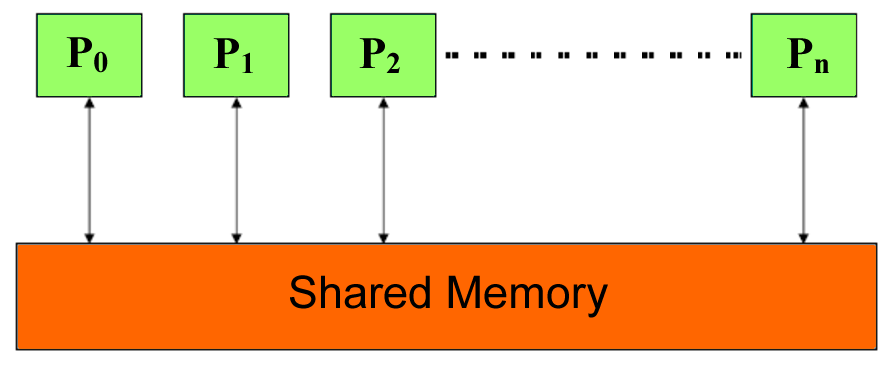
\includegraphics[scale=.6]{./images/Pram.png}
\caption{PRAM  model (\textit{Parallel Random Access Machine.})}
\label{fig:Pram}
\end{figure}

The advantage of the PRAM model is its simplicity and its similarity to the sequential model of von Neumann. The processor can only read or write a memory address in one cycle. The cost of writing is equal to the cost of reading, and is also equal to the cost of any operation performed by the processor. However, in spite of its simplicity, due to the increase in the distance between the processing and the speed of communication, this model has become more and more unrealistic.

Different submodels were created from the PRAM model. Researchers have made adaptations varying the way of access to memory, trying to avoid the maximum of conflicts in the communication. The different adaptations have arisen to propose concurrent or exclusive communications at the moment to access to shared memory~\citep{Gibbons19983:QRQW, Karp:CSD-88-408}. 

\subsection{Bulk Synchronous Parallel Model (BSP)}
The BSP model was introduced by~\cite{Valiant:1990}. The BSP model offers a simple abstraction of parallel architectures, see Figure \ref{fig:BSP}. In Figure~\ref{fig:BSP} a set of processors are running local computations in a superstep and before the synchronization, all the messages are delivered and ready to be used in the next superstep.

\begin{figure}[htpb]
\centering
% 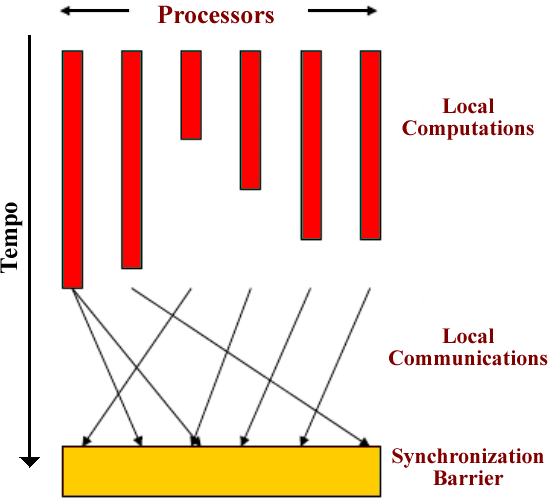
\includegraphics[scale=.7]{./images/bspmodel.eps}
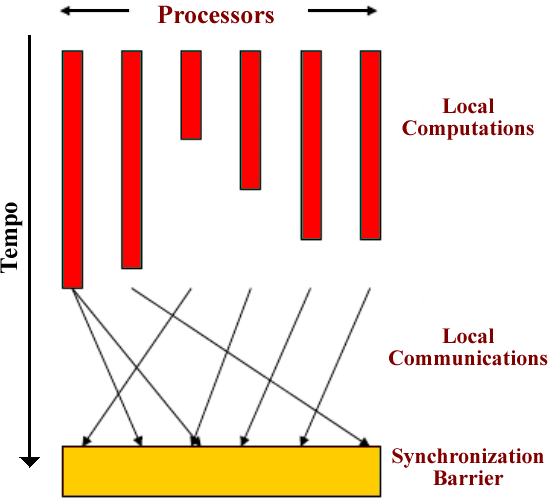
\includegraphics[scale=.7]{./images/bspmodel.png}
\caption{Superstep in a Bulk Synchronous Parallel Model.}
\label{fig:BSP}
\end{figure}

The BSP model bridges the essential characteristics of different kinds of machines as a combination of three attributes:

\begin{itemize}
\item a set of virtual processors, each associated to a local memory;
\item a router, that delivers the messages in a point-to-point manner;
\item a synchronization mechanism.
\end{itemize}

The execution of a parallel application is organized in a sequence of \emph{supersteps}, each one divided into three successive---logically disjointed---phases.
On the first phase, all processors use their local data to perform local sequential computations in parallel (i.e., there is no communication among the processors). The second phase is a communication phase, where all nodes exchange data performing personalized all-to-all communication. The last phase consists of a global synchronization barrier, that guarantees that all messages were delivered and all processors are ready to start the next superstep. 

Figure~\ref{fig:BSP} depicts the phases of a BSP application. In this figure, a processor distributes tasks to a set of processors that execute local computations and communicate in a global form, if necessary. All processors wait for the others finish their tasks in a synchronization barrier, to be able to execute the next task. Sending and receiving messages between processors is only allowed at the end of each super-step.

On the BSP model there is no restriction on sending messages, but all of them should be received before the synchronization barrier. According to the execution model, the first and second phase may occur simultaneously. A BSP algorithm consists of an arbitrary number of super-steps. The BSP model has been widely used on different applications contexts. HPC practitioners have been using the BSP model to design algorithms and software that can run on any standard architecture with guaranteed performance \cite{AlgGPU,Goldberg2004,CamargoGKG06}. Consider a BSP program that runs on $S$ supersteps. Let $g$ be the bandwidth of the network and $L$ the latency---i.e., the minimum duration of a superstep---which reflects not only the latency of the network, but also the overhead of the synchronization step. The cost to execute the $i$-th superstep is then given by:

\begin{equation}
  \label{eq:superstep-cost}
  w_i + g h_i + l
\end{equation}

where $w_i$ is the maximum amount of local computations executed, and $h_i$ is the largest number of packets sent or received by any processor during the superstep. If $W = \sum_{i=1}^{S} w_i$ is the sum of the maximum work executed on all supersteps and $H = \sum_{i=1}^{S} h_i$ the sum of the maximum number of messages exchanged in each superstep, then the total execution time of the parallel application is given by:
\begin{equation}
  \label{ec:BSP}
  T = W + g H + L S
\end{equation}

A BSP algorithm, consequently, can be completely modeled by the parameters $(w, h, g, l)$. Using these parameters, the approximate execution time of a BSP algorithm can be characterized. One of the great advantages of the BSP model is that it facilitates to develop parallel programs on different systems and architectures, serving as a bridge between the programmer who develop parallel applications in massively parallel architectures.

\subsubsection{Multi-BSP model}
The Multi-BSP model is an adaptation of the BSP model, the BSP model is commonly used in a distributed memory parallel environment, and multi-BSP is a BSP extension for multi-core processors. ~\cite{Valiant:2011} created the Multi-BSP model which is used in a parallel shared memory environment. Computational models, such as multi-BSP, allow abstraction of the complexity of the problem in a simplification that is not significantly away from the reality of current computational  architectures.  

Multi-BSP is a multi-level model that has explicit parameters at each level: number of processors $p$, memory/cache sizes $m$, communication latency costs $g$ and synchronization costs $L$. The multi-BSP model of an architecture with depth $d$ will be determined by $4d$ numeric parameters, $(p1, g1, L1, m1), (p2, g2, L2, m2), ( P3, g3, L3, m3), ..., (pd, gd, Ld, md)$. At each level the four parameters quantify, respectively, the number of subcomponents, processors, communication bandwidth, synchronization cost, and memory/cache size~\citep{BSPMeasures}.

Multi-BSP and BSP are important models that allow bridging the analysis, design and development of parallel algorithms, but they are not useful to design algorithms that are executed in massively parallel architectures. New models of performance prediction of applications that run on GPUs have arisen from adaptations of the models in this literature review.

\subsection{Coarse Grained Multicomputer Model (CGM)}
\cite{Dehne:2002} studied the problem of designing scalable parallel geometric algorithms for coarse grained cases. They called this model as Coarse Grained Multicomputer model (CGM), which is very efficient for a large set of problems of the ratio $\frac{n}{p}$, with $n$ the size of the problem and $p$ the number of processors. In other words, the CGM model is very good for addressing problems where the problem of size $n$ can be divided between an determined number of processors $p$. A CGM algorithm is a special case of a BSP algorithm where all communication operations of a super-step are done in $h$ relations. A fundamental difference between the BSP model and CGM is that the first captures real machine parameters while the CGM is an abstraction that allows to develop efficient algorithms in parallel machines.

An algorithm on a CGM machine can be modeled using only two parameters, $N$ and $p$. This algorithm consists of an alternating sequence of computing and communication rounds also separated by a synchronization barrier. A computational/communication round of the CGM model corresponds to a super-step of the BSP model with communication cost $g(N/p)$. A good performance of algorithms with the CGM model is achieved by minimizing the number of super-steps, the total time of local computations and the total size of the messages.

\subsection{LogP Model}
Synchronization of a large group of processes or threads is expensive in terms of latency, especially on architectures with classification MIMD. For these cases, parallel computing models without synchronization were created. The most popular of these models is the logP model.

LogP model was proposed by \citet{Culler:1993:LogP} and received its name exactly for the variables of the model. Culler et. al. perceived that the PRAM model was not realistic due to the lack of parameters to represent communication costs in parallel applications, especially for distributed applications. The parameters used to describe a parallel system according to LogP model are:

\begin{itemize}
\item[L:] \textit{Latency} - caused by communicating a message from a source to a destiny processor.
\item[o:] \textit{Overhead} - time during which a processor is busy sending or receiving a message, during that time it can not do
computations.
\item[g:] \textit{Gap} - minimum time between consecutive message transmissions or between receiving consecutive messages; the reciprocal of $g$ corresponds to the bandwidth of the system.
\item[P:] \textit{Processors}.
\end{itemize}


\section[BSP-based model to predict execution time of CUDA Kernels]{A Simple BSP-based model to predict execution time of CUDA Kernels}\label{sec:proposeModel}

In this section we propose a novel simple BSP-model to predict execution time of CUDA kernels executed over GPUs. Similarly to the BSP model, our model is mainly based on the number of computational and communication steps used by the application. These values are multiplied by parameters that describe the number of cores, threads and the clock rate of the processors. Differently from the BSP model, we did not include the synchronization step of the BSP model, since global synchronizations in GPUs occur only at the end of the kernel. This model takes into account the main physical properties and optimizations of GPU architectures. The performance prediction is based on the cost of communication and computation, which are determined independently. The execution time is split between computation and data transferring to and from global and shared memories. 

\begin{equation}\label{ec:BSPGPU}
t_k = \frac{t \cdot (Comp + Comm_{GM} + Comm_{SM})}{R \cdot P \cdot \lambda}
\end{equation} 

In Equation~\ref{ec:BSPGPU}, $t_k$ is the approximated execution time of a kernel function with $t$ threads. It sums the computational cost ($Comp$) with the communication cost of global memory ($Comm_{GM}$) and shared memory ($Comm_{SM}$) accesses, performed by each thread. This cost is multiplied by the number of threads $t$ and divided by the clock rate $R$ times the number of cores $P$ available in the GPU. The parameter $\lambda$ is used to model the effects of application optimizations, such as divergence, shared bank conflicts and coalesced global memory accesses.

The computational time used by each thread in a kernel is denoted by $Comp$. It is determined by the number of cycles that each thread spends in its computation. FMA operations can be included in $Comp$ by reading the source code of the kernel and verifying this possibility with profiling tools. 

Communication is evaluated at two levels: global and shared memory. The execution time for communication in global and shared memory per thread are given by $Comm_{GM}$ and $Comm_{SM}$, respectively. These are defined as the sum of load and write transactions over the global memory and shared memory. This information can be extracted directly from the source code. %Shared memory is on chip in each multiprocessor and has a very small latency in this memory level on chip has zero-overhead.

Additionally, to account the effects of cache memories on recent GPU architectures, the number of L1 and L2 cache hits are subtracted from the number of loads over the global memory. We have used metrics and events to confirm information about the number of L1 and L2 cache hits. Their contribution to the execution time is calculated separately, multiplying them by their latency times~\citep{GPU:BenchMark, Bench:GPU}. This model allows an easy parametrization, well-suited for any GPU applications in practice. For simplification, we do not consider  constant and texture memories nor differences between the latency of load and store transactions. $Comm_{SM}$ and $Comm_{GM}$ are defined as:

\begin{equation}\label{ec:SM}
Comm_{SM} = \left(ld_{0} + st_{0} \right) \cdot g_{SM}
\end{equation}


\begin{equation}\label{ec:GM-cache}
Comm_{GM} = \left(ld_{1} + st_{1} - L1 - L2 \right) \cdot g_{GM} + L1\cdot g_{L1} + L2\cdot g_{L2} 
\end{equation}

$g_{GM}$, $g_{SM}$, $g_{L1}$ and $g_{L2}$ represent the latency in communication over global, shared, L1 cache and L2 cache memory, respectively. Some typical values are $5$ cycles for $g_{SM}$ and $g_{L1}$, $500$ cycles for $g_{GM}$ \citep{CUDA:Best}, and 250 cycles for $g_{L2}$. When the L1 and/or L2 caches are enabled for catching. 

When the application reaches a stable access on L2 cache and L1 cache is disabled for catching the equation~\ref{ec:GM-cache} can be expressed for the equation~\ref{ec:GM}. When the executions are stables, the cache utilization keeps regular with the problem size of the application. 

\begin{equation}\label{ec:GM}
Comm_{GM}  = \left(ld_{1} + st_{1} \right) \cdot g_{GM} 
\end{equation}

$ld_{0}$ and $st_{0}$ represent the total number of load and stores performed by all threads in the shared memory, and $ld_{1}$ and $st_{1}$ represent the loads and stores for global memory. The number of loads and stores to global and shared memory are determined by analyzing the CUDA source code. $L1$ and $L2$ are determined executing an application execution profile and taking the number of hits over each one of these memory levels. 

Aspects about optimization of CUDA kernels, such as coalesced accesses, shared bank conflicts and divergence are important to define the performance of a kernel~\citep{Wu:2013:Coalesced}. We consider the effects of those optimizations using the $\lambda$ factor.  It is estimated as the ratio between the predicted execution time of the kernel with the actual measured execution time. The $\lambda$ factor is important since it permits the adjustment of application performance with the implemented CUDA optimizations and GPU architectures. Finally, intra-block synchronization is not computed, since it does not affect processing time~\citep{CUDA:Best,GpuNOsynchronize}. Intra-block synchronization is very fast, and did not need to be included. Nevertheless, we maintained the inspiration on the BSP-model because the extended version of the model considering host memory needs global synchronizations.

Consequently, except for the value of $\lambda$ and effects on caches L1 and L2, all other parameters are constants. The effect of usage of caches L1 and L2 must be confirmed by profiling. $\lambda$ performs the adjustment of application performance with the implemented CUDA optimizations. Once defined for the application, the same relative value should work for other similar GPUs and input sizes of the application. 

Next section will show how each one of the parameters were obtained from each one of the CUDA kernels of the testbed.

\section{Methodology}\label{sec:methodModel}
We have tested the model with all applications presented in Table~\ref{tab:useCases}, all of them in CUDA using the single-precision format and running a single kernel. These are: \emph{Matrix Multiplication}, \emph{Matrix Addition}, \emph{dot product}, \emph{Vector addition} and \emph{Maximum Subarray Problem} \citep{Cleber:Thesis}. For \emph{matrix multiplication}, we have used 4 different kernel strategies, and for \emph{matrix addition} we have used 2 kernel strategies. In total, we have used 9 different CUDA kernels of those matrix and vector GPU applications. The number of computation ($Comp$) and communication ($ld_0$, $st_0$, $ld_1$ and $ld_1$) steps were extracted from the application source codes, and information about cache hits in cache L1 and L2 were extracted from profiling. We also confirmed the usage of FMA and SFU using profiling. 

We have also used 6 kernels of the Rodinia applications, these kernels belong to 4 different GPU applications. These applications are: Back-propagation, Gaussian Elimination, Heartwall and Hotspot. There are applications which each execution generate one execution of the kernel and consequently a sample for our experiemnts, these are all in Table~\ref{tab:useCases} and both in the application Back propagation. Each execution of the other Rodinia applications generate multiples execution of their kernels and thus multiples samples for our experiments. During our evaluations, all applications were executed using the CUDA profile tool \textit{nvprof}. Each experiment is presented as the average of ten executions, with a confidence interval of 95\%. Only Rodinia Applications were executed on GPU Pascal. 


\textbf{\emph{Vector-Matrix Applications}}\\


For the analytical model, 69 samples of each application for problems of one dimension were taken from $2^{17}$ until $2^{28}$. From $2^{17}$ to $2^{22}$ 6 samples were taken, and from $2^{23}$ to $2^{28}$ 63 samples were collected. 32 samples of each application for problems of two dimensions were taken from $2^8$ until $2^{13}$, the input sizes or matrix sizes were vary increasing the matrix size in a step of $2^8$. Each one of the parameters of the BSP-based model were extracted from the source code of each kernel.  

For matrix multiplication versions, $Comp$ is determined by the number of multiplications and/or operations computed by a thread. In this case, each thread performs $N$ FMA single precision operations. IEEE~754-2008 floating-point standard~\citep{FMA-IEEE} states that those operations needs a single rounding step. The value of $Comp$ is the same for the all four optimizations modes, since they differ only in the memory access patterns. With those values, we can compute ---using equations \ref{ec:GM} and \ref{ec:SM}--- the values of $Comp$, $Comm_{GM}$, and $Comm_{SM}$, that are then multiplied by the number of threads $t$ in the kernel execution. 

The optimizations actually affect only the performance of the communication between threads. As explained above, $\lambda=1$ in the first execution and it is obtained by the ratio of the predicted execution time of the application with the actual measured execution time. The parameter $\lambda$ captures the effects of thread divergence, global memory access optimizations, and shared memory bank conflicts. It needs to be measures only once, for a single input size and a single board. The same lambda should work for all input sizes and boards of the same architecture. These parameters are the same for all the simulations, and are presented in Table \ref{tab:Par-NCA}.

As it was explained in Section~\ref{ssec:useCases}, each thread in both version of matrix addition request 1 element from each matrix elements and compute a single addition. The values of the parameters of the model for (MAU) and (MAC) is $Comp=1add$, $ld_1=2$, $st_1=1$, $ld_0=0$ and $st_0=0$. In the same way the parameter values of the model for (vAdd) were determined. 

The kernel of the Maximum Sub-Array Problem (MSA) is implemented using the CGM model, however it can be easily modeled with the proposed model. The scalability  of this application is also very regular. Despite the branch code divergence in the source code of this kernel, this scalability is not altered. This kernel is computed with 4096 threads, divided in 32 thread blocks with 128 threads on each. The $N$ elements are divided in intervals of $N/t$ elements, one per block and each block receive a portion of the array. The blocks use the shared memory for storing segments of its interval, which are read from the global memory using coalesced accesses.The values of the parameters of the model for (MSA) are shown in Table~\ref{tab:Par-NCA}.

\begin{table}[htpb]
\centering
\scalebox{.8}{
\begin{tabular}{| c | c | c  |  c | c | c | c | c | c | c |} 
\midrule
\multirow{2}{*}{\textbf{Par.}} & \multicolumn{4}{c|}{\textbf{Matrix 
Multiplication}}&\multicolumn{2}{c|}{\textbf{Matrix 
Addition}}&\multirow{2}{*}{\textbf{vAdd}}&\multirow{2}{*}{\textbf{dotP}}&\multirow{2}{*}{\textbf{MSA}}
\\\cline{2-7}&\textbf{MMGU}&\textbf{MMGC}&\textbf{MMSU}&\textbf{MMSC}&\textbf{MAU}&\textbf{MAC}&&\\\midrule
$\mathbf{comp}$&\multicolumn{4}{c|}{$N\cdot$ FMA}&\multicolumn{3}{c|}{$1\cdot 24$}&$1\cdot 96$&$(N/t)\cdot{}100 $\\\midrule
$\mathbf{ld_1}$&\multicolumn{4}{c|}{$2\cdot N$}&\multicolumn{3}{c|}{2}&2&$N/t$\\\midrule
$\mathbf{st_1}$&\multicolumn{4}{c|}{1}&\multicolumn{3}{c|}{2}&$1/GS$&$5$\\\midrule
$\mathbf{ld_0}$&\multicolumn{2}{c|}{0}&\multicolumn{2}{c|}{$2\cdot N$}&\multicolumn{3}{c|}{0}&$1 + 2\cdot{}log(BS)$&$2\cdot{}(N/t)$\\\midrule
$\mathbf{st_0}$&\multicolumn{2}{c|}{0}&\multicolumn{2}{c|}{1}&\multicolumn{3}{c|}{0}&$1 + 2\cdot{}log(BS)$&$N/BS^2$\\
\midrule
\end{tabular}}
\caption{Values of the model parameters over 9 different vector/matrix applications}
\label{tab:Par-NCA} % is used to refer this table in the text
\end{table}

Different micro-benchmarks were used to measure the number of cycles per computation operation in GPUs~\citep{Bench:GPU}, with FMAs, additions, multiplications, divisions,  taking approximately 8, 16, 32 and up to 96 cycles of clock. For all simulations, we considered $5$ cycles for latency in the communication for shared memory and $500$ cycles for global memory \citep{CUDAGuide}. Finally, when the models were complete, we executed a single average instance of each application on each GPU to determine the $\lambda$ values. As explained above, $\lambda=1$ in the first execution and it is obtained by the ratio of the predicted execution time of the application with the actual measured execution time. Finally, for the parameter $\lambda$, which captures the effects of thread divergence, global memory access optimizations, and shared memory bank conflicts, we used the values described in Table~\ref{tab:Lambda-NCA}. 

\begin{table}[htpb]
\centering
\scalebox{0.8}{
\begin{tabular}{| c | c | c  |  c | c | c | c | c | c | c |} 
\hline \hline
\multirow{2}{*}{\textbf{\backslashbox{GPUs}{Kernels}}}& \multicolumn{4}{c|}{\textbf{Matrix Multiplication}}& \multicolumn{2}{c|}{\textbf{Matrix Addition}}&\multirow{2}{*}{\textbf{vAdd}}&\multirow{2}{*}{\textbf{dProd}}&\multirow{2}{*}{\textbf{MSA}} \\\cline{2-7}
&\textbf{MMGU}&\textbf{MMGC}&\textbf{MMSU}&\textbf{MMSC}&\textbf{MAU}&\textbf{MAC}\\\hline
GTX-680 &\cellcolor{green!50} 4.50 &\cellcolor{green!50} 19.00 &\cellcolor{green!50} 20.00 &\cellcolor{green!50} 68.00 &\cellcolor{green!50} 1.50 &\cellcolor{green!50} 9.25 &\cellcolor{green!50} 14.00 &\cellcolor{green!50} 11.00 &\cellcolor{green!50} 0.68 \\ 
  Tesla-K40 &\cellcolor{green!50} 4.30 &\cellcolor{green!50} 20.00 &\cellcolor{green!50} 19.00 &\cellcolor{green!50} 65.00 &\cellcolor{green!50} 2.50 &\cellcolor{green!50} 9.50 &\cellcolor{green!50} 5.50 &\cellcolor{green!50} 10.00 &\cellcolor{green!50} 0.48 \\ 
  Tesla-K20 &\cellcolor{green!50} 4.50 &\cellcolor{green!50} 21.00 &\cellcolor{green!50} 18.00 &\cellcolor{green!50} 52.00 &\cellcolor{green!50} 2.50 &\cellcolor{green!50} 9.00 &\cellcolor{green!50} 6.00 &\cellcolor{green!50} 10.00 &\cellcolor{green!50} 0.55 \\ 
  Titan &\cellcolor{green!50} 4.25 &\cellcolor{green!50} 21.00 &\cellcolor{green!50} 17.00 &\cellcolor{green!50} 50.00 &\cellcolor{green!50} 2.50 &\cellcolor{green!50} 10.00 &\cellcolor{green!50} 5.50 &\cellcolor{green!50} 12.00 &\cellcolor{green!50} 0.48 \\ 
Quadro &\cellcolor{green!50} 4.75 &\cellcolor{green!50} 20.00 &\cellcolor{green!50} 20.00 &\cellcolor{green!50} 64.00 &\cellcolor{green!50} 1.50 &\cellcolor{green!50} 8.25 &\cellcolor{green!50} 11.00 &\cellcolor{green!50} 9.50 &\cellcolor{green!50} 0.55 \\
  TitanX & 9.50 & 36.00 & 36.00 & 110.00 & 3.00 & 9.50 & 7.00 & 9.75 & 0.95 \\ 
  GTX-970 & 13.00 & 44.00 & 46.00 & 120.00 & 3.75 & 9.50 & 8.00 & 10.50 & 1.95 \\ 
  GTX-980 & 13.00 & 44.00 & 46.00 & 120.00 & 3.25 & 9.50 & 7.00 & 9.50 & 1.50 \\\hline
\end{tabular}}
\caption{Values of the parameter $\lambda$ for each vector/matrix CUDA kernel in the GPUs used}
\label{tab:Lambda-NCA} % is used to refer this table in the text
\end{table}

The Values of $\lambda$ for each application and each GPU is shown in Table~\ref{tab:Lambda-NCA} and graphically in Figure~\ref{fig:LambdaNCA}. Green Cells in Table~\ref{tab:Lambda-NCA} groups the values of $\lambda$ by GPU architectures, those without color belong to Maxwell architecture and those of green are Kepler architectures. The same lambda should work for all input sizes and boards of the same architecture. The box plots of Figure~\ref{fig:LambdaNCA} show the median for each application in all the GPUs and the upper and lower first quartiles, with whiskers representing the 95\% confidence interval. Outliers are marked as individual points.

\begin{figure}[htpb]
\centering
 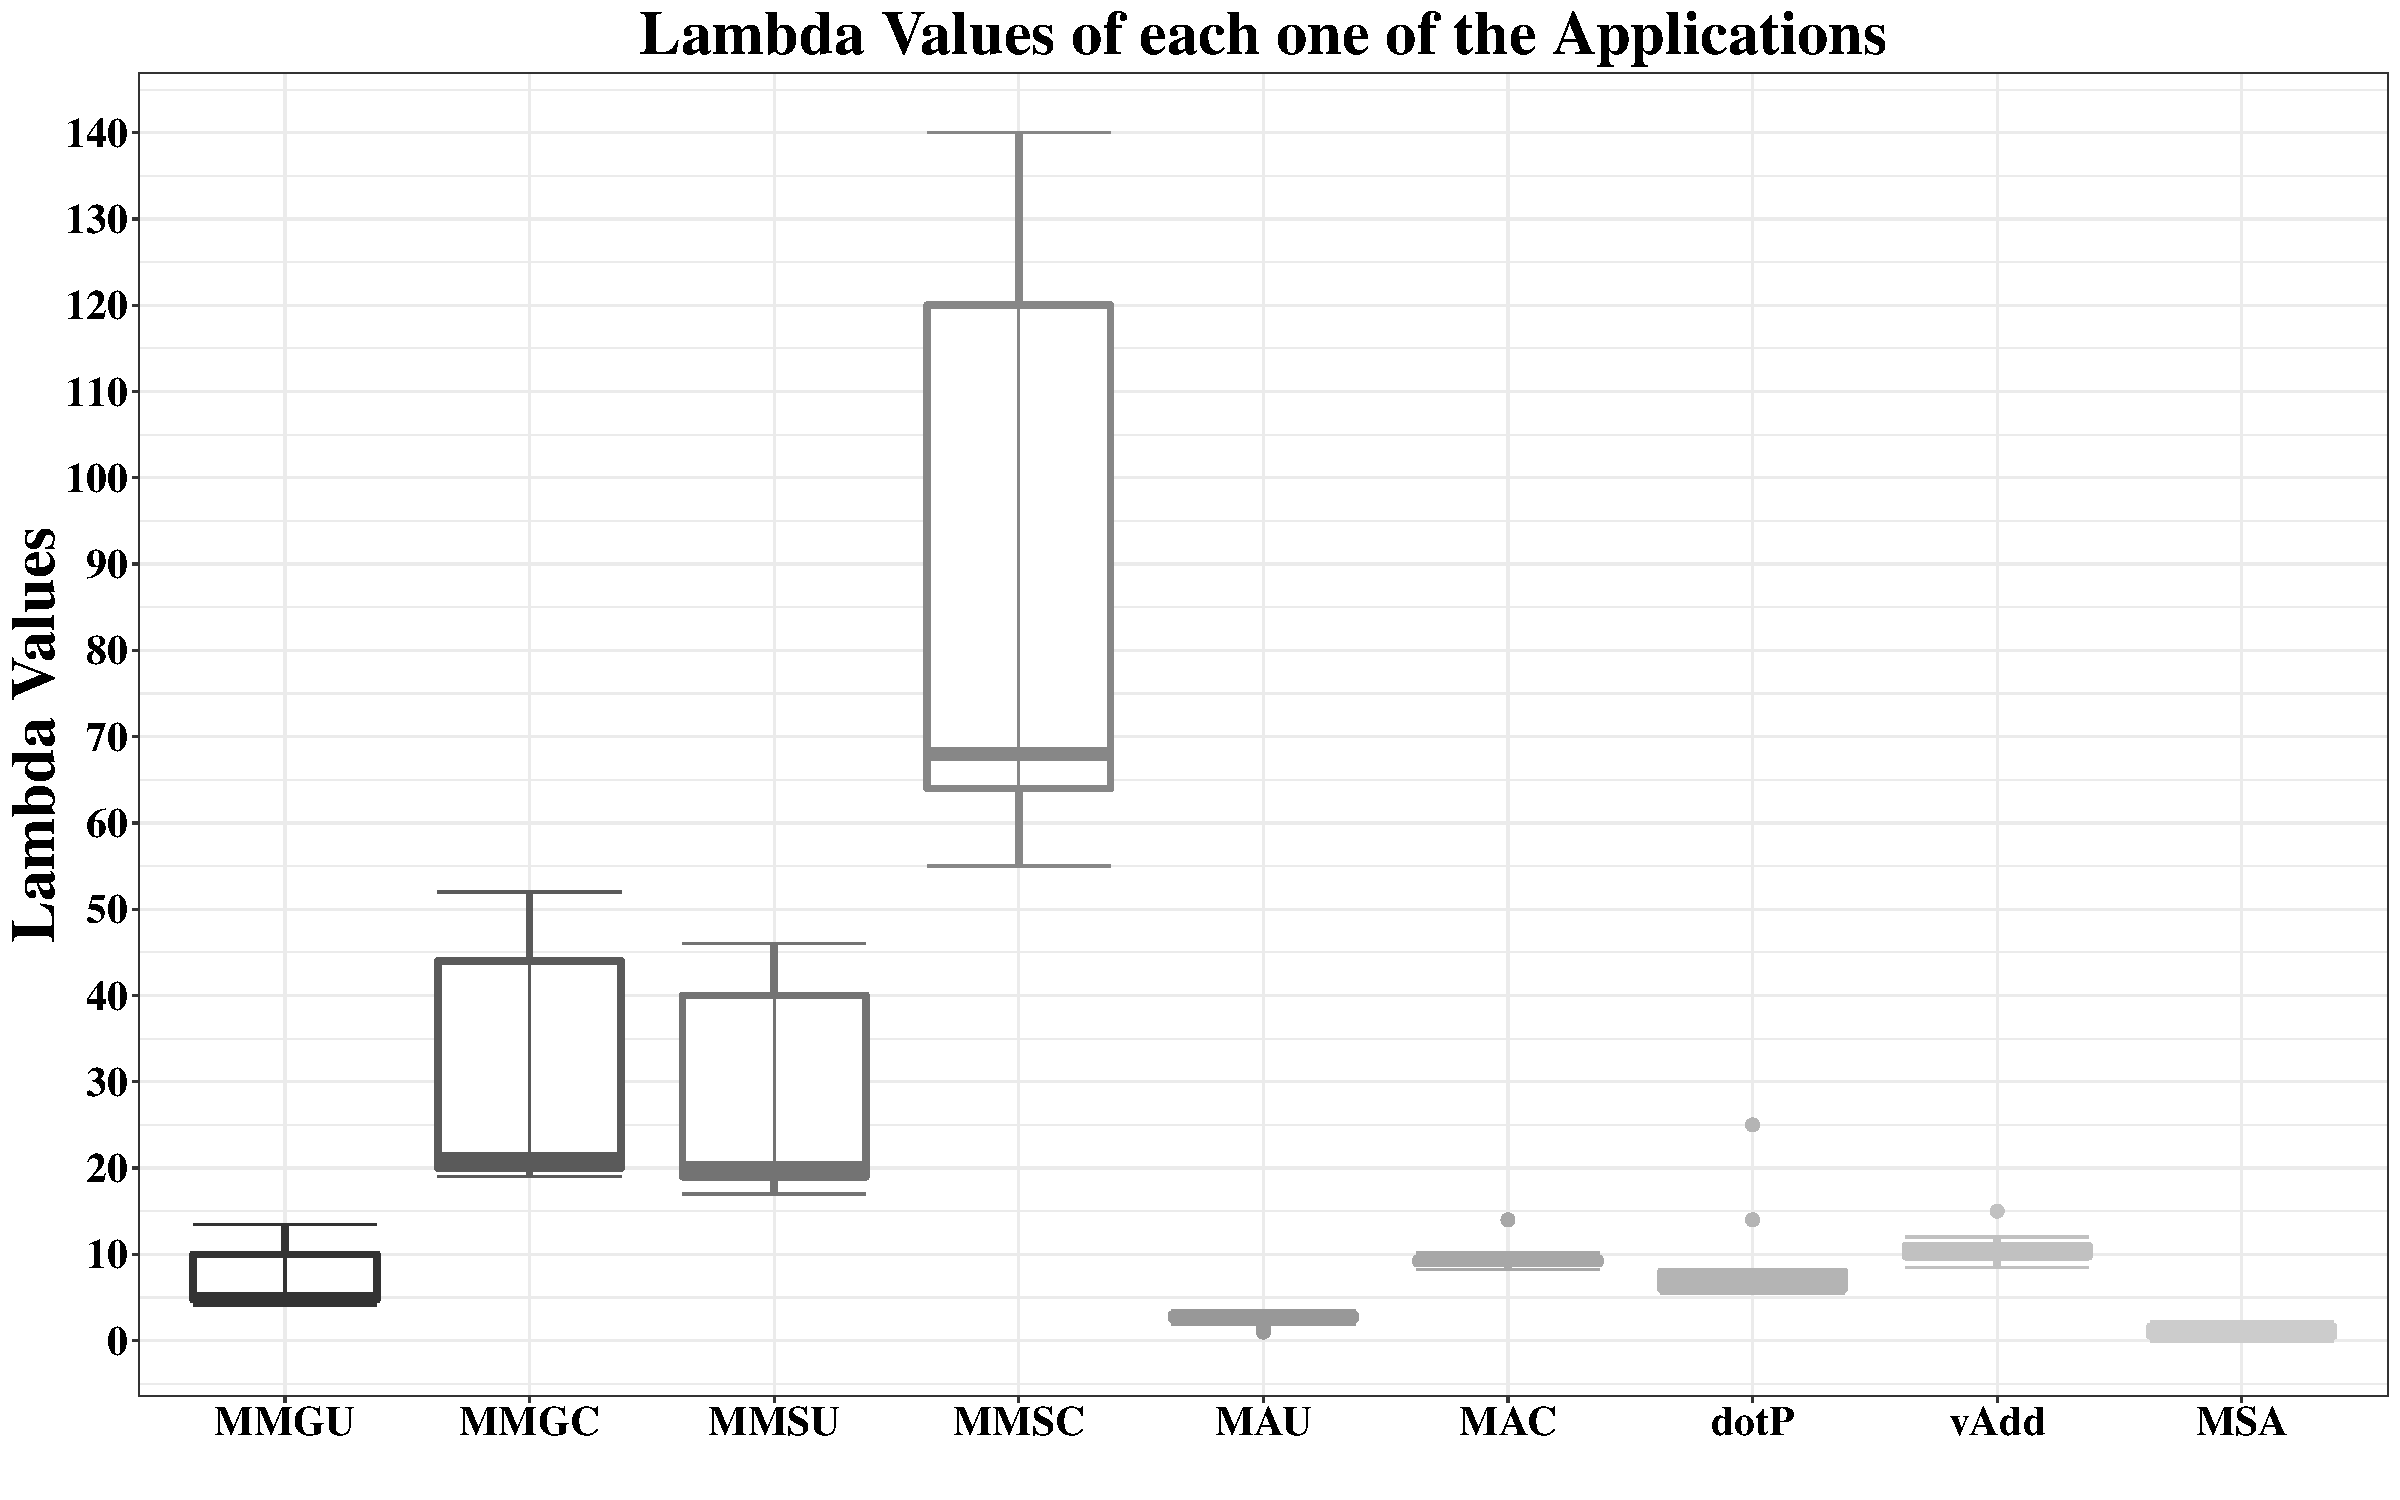
\includegraphics[scale=.3]{./images/LambdaAnalyticalModel-NCA.pdf}
\caption{Boxplot of $\lambda$ values, see table~\ref{tab:Lambda-NCA}}
\label{fig:LambdaNCA}
\end{figure}

\textbf{\emph{Rodinia Benchmark Applications}}\\
Our analytical model was tested with 4 Rodinia algorithms, Back-propagation, Gaussian Elimination, Heartwall and Hotspot. The number of samples of each application is shown in Table~\ref{tab:Rodinia}. Similarly to the vector/matrix applications mentioned before, the variables of computation ($Comp$) and communication ($ld_0$, $st_0$, $ld_1$ and $ld_1$) were extracted from the application source codes. For kernel (HWL), it was not possible to know the values of the parameters of the analytical model, due to the large number of code lines. For this reason the values of the parameters for the analytical model were extracted from profile information. These values are presented in Table~\ref{tab:Par-Rodinia}.  Kernel (HWL) uses constant memory to store large numbers of parameters which cannot be readily fit into shared memory, resulting in a high number of instructions over the global memory. Finally, when values of the parameters of the models were completed, we executed a single instance of each application on each GPU to determine the $\lambda$ values. As explained above, $\lambda=1$ in the first execution and it is obtained by the ratio of the predicted execution time of the application with the actual measured execution time. 

\begin{table}[htpb]
\centering

\begin{tabular}{| c | c | c  |  c | c | c | c |} 
\midrule
\multirow{2}{*}{\textbf{Par.}} & \multicolumn{2}{c|}{\textbf{Back propagation}}&\multicolumn{2}{c|}{\textbf{Gaussian}}&\multirow{2}{*}{\textbf{HWL}}&\multirow{2}{*}{\textbf{HOT}}
\\\cline{2-5}& \textbf{BCK-1} & \textbf{BCK-2} & \textbf{GAU-1} & \textbf{GAU-2} & &   \\\midrule
$\mathbf{comp}$&404&116&36&96&7600000&500 \\\midrule
$\mathbf{ld_1}$&2&4&1&3&7000&2\\\midrule
$\mathbf{st_1}$&1/GS&1&1&1&2000&1\\\midrule
$\mathbf{ld_0}$&BS&0&0&0&2800&2\\\midrule
$\mathbf{st_0}$&BS&0&0&0&1&1\\
\midrule
\end{tabular}
\caption{Values of the model parameters over 6 CUDA kernels of Rodinia Benchmark Suite}
\label{tab:Par-Rodinia} % is used to refer this table in the text
\end{table}

Finally, for the parameter $\lambda$ of the Rodinia CUDA kernel, which captures the deep thread and memory hierarchy, we used the values described in Table~\ref{tab:lambdaRodinia}. These values are also shown graphically in Figure~\ref{fig:LambdaRodinia}. This table present three different groups, they are green, blue and without color, which group GPU architecture which are Kepler, Maxwell and Pascal architectures, respectively. It is easy also to notice that values of the $\lambda$ parameter have less variance when belong to the same architecture.



\begin{table}[htpb]
\centering
\begin{tabular}{|r|c|c|c|c|c|c|}
  \hline
 \textbf{\backslashbox{GPUs}{Kernels}}& BCK-1 & BCK-2 & GAU-1 & GAU-2 & HWL & HOT  \\ 
  \hline
    GTX-680 &\cellcolor{green!50} 6.2 &\cellcolor{green!50} 7.50 &\cellcolor{green!50} 0.26 &\cellcolor{green!50} 0.65 &\cellcolor{green!50} 2.15 &\cellcolor{green!50} 8.00 \\ 
  Tesla-K40 &\cellcolor{green!50} 6.30 &\cellcolor{green!50} 8.50 &\cellcolor{green!50} 0.35 &\cellcolor{green!50} 1.25 &\cellcolor{green!50} 2.25 &\cellcolor{green!50} 14.00 \\ 
  Tesla-K20 &\cellcolor{green!50} 6.4 &\cellcolor{green!50} 8.50 &\cellcolor{green!50} 0.35 &\cellcolor{green!50} 1.25 &\cellcolor{green!50} 2.50 &\cellcolor{green!50} 14.50 \\ 
  Titan &\cellcolor{green!50} 6.2 &\cellcolor{green!50} 8.50 &\cellcolor{green!50} 0.35 &\cellcolor{green!50} 1.25 &\cellcolor{green!50} 2.25 &\cellcolor{green!50} 14.00 \\ 
  Quadro &\cellcolor{green!50} 5.60 &\cellcolor{green!50} 7.00 &\cellcolor{green!50} 0.25 &\cellcolor{green!50} 0.70 &\cellcolor{green!50} 1.65 &\cellcolor{green!50} 8.00 \\ 
  TitanX &\cellcolor{blue!25} 4.20 &\cellcolor{blue!25} 5.50 &\cellcolor{blue!25} 0.40 &\cellcolor{blue!25} 2.00 &\cellcolor{blue!25} 3.25 &\cellcolor{blue!25} 7.00 \\ 
  GTX-970 &\cellcolor{blue!25} 5.60 &\cellcolor{blue!25} 6.50 &\cellcolor{blue!25} 0.70 &\cellcolor{blue!25} 3.50 &\cellcolor{blue!25} 5.00 &\cellcolor{blue!25} 8.00 \\ 
  GTX-980 &\cellcolor{blue!25} 4.5 &\cellcolor{blue!25} 5.75 &\cellcolor{blue!25} 0.45 &\cellcolor{blue!25} 2.50 &\cellcolor{blue!25} 3.75 &\cellcolor{blue!25} 7.00 \\
  Tesla-P100 & 8.40 & 10.50 & 0.30 & 2.00 & 5.50 & 25.00 \\ 
   \hline
\end{tabular}
\caption{Values of the parameter $\lambda$ for each Kernels of the Rodinia Benchmark in the GPUs used}
\label{tab:lambdaRodinia}
\end{table}

In all experiments, we modeled only communication over global memory and shared memory. We did not include the values of the cache L2 for these experiments because they did not impact the variance of the execution times. And $L1$ caching in Kepler, Maxwell and Pascal architectures is reserved for register spills in local memory. For this reason $L1$ and $L2$ are always 0 for all the experiments. Cache effects are hard to predict and its impact is higher for specific applications and problem sizes. For example, small vector/matrix problems can profit more from L1 cache memory. This happens in applications which do not use shared memory and their accesses to the global memory are uncoalesced, since they can exploit the cache line size and load multiple elements in the same transaction~\citep{Wu:2013:Coalesced}.

\begin{figure}[htpb]
\centering
 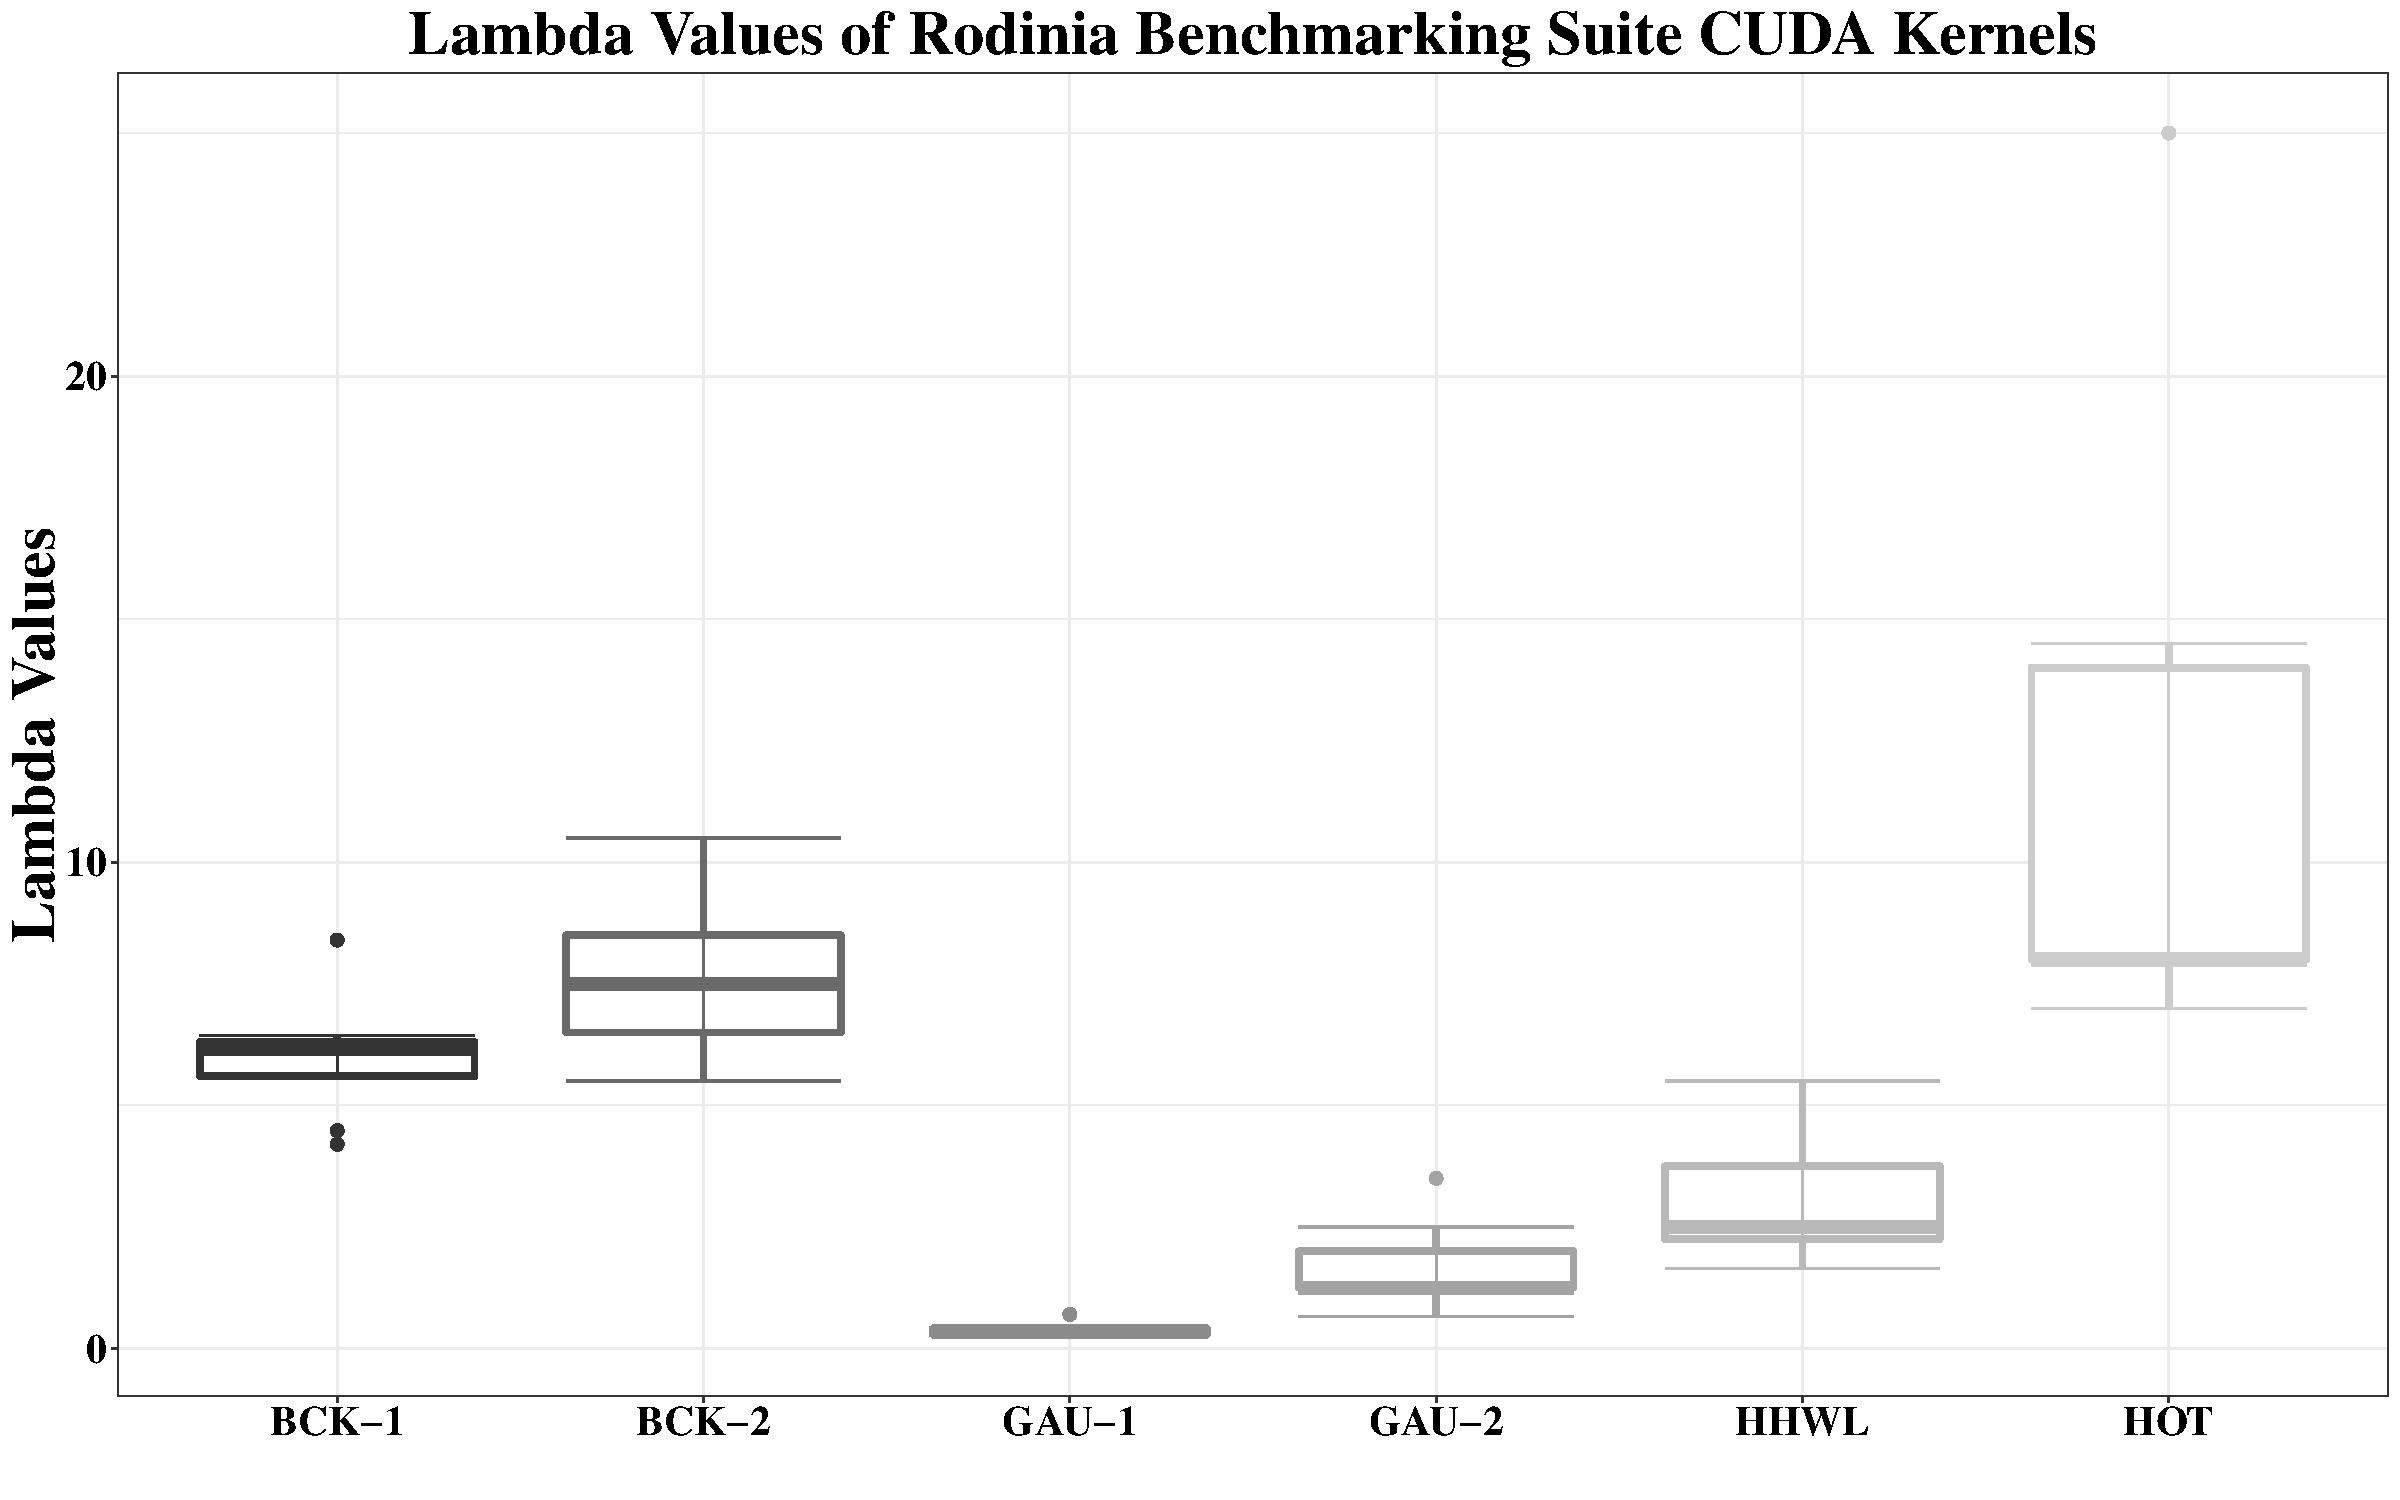
\includegraphics[scale=.3]{images/LambdaAnalyticalModel-Rodinia.pdf}
\caption{Boxplot of $\lambda$ values of Rodinia CUDA Kernels, see table~\ref{tab:lambdaRodinia}}
\label{fig:LambdaRodinia}
\end{figure}
% Note that higher optimizations levels results in larger $\lambda$ values and, consequently, the $\lambda$ can bwe considered an estimator of the application optimization level. 

We have used our analytical model in some Rodinia Applications, for them which the analytical model was adequate. The proposed BSP-based analytical model is useful for those applications which its scalability is regular with the input parameters. When kernels iterate in an application and the number of threads and divergence change on each iteration, it makes difficult to predict the running time of different CUDA kernels. Machine learning can be a solution for this type of kernels, in Chapter~\ref{Chap:ML} we describe a implementation of machine learning techniques for these kernels in two different approaches. Another option would be to use other analytical models which are explained in Section~\ref{sec:relatedModel} of this chapter.



%=============================================================================
\section{Experimental Results}\label{sec:resultModel}

We used $T_k$ values computed as described in Section~\ref{sec:proposeModel}. We have performed experiments to evaluate the predictions of our model, by comparing these predictions with measurements of executions of the applications over different GPUs showed in Table~\ref{tab:GPUs}. For all simulations, we considered $5$ cycles for latency in the communication in shared memory and $500$ cycles are considered for latency communication in global memory \citep{CUDA:Best}. Finally, for the parameter $\lambda$, which captures the effects of thread divergence, global memory access optimizations, and shared memory bank conflicts, we used the values described in the previous section. We compared the measured times ($T_m$) with the times predicted by the proposed model ($T_k$), and used the ratio $T_k/T_m$ to define the precision of the prediction. 

Figure~\ref{fig:resultsVMApp} and \ref{fig:ResultsRodinia} show the obtained results for the vector/matrix applications and some Rodinia Kernels. These figures show the box plots of the accuracy of the BSP-based analytical model over the different selected CUDA kernels. The box plots show the median for each GPU and the upper and lower first quartiles, with whiskers representing the 95\% confidence interval. Outliers are marked as individual points. For vector/matrix applications in the \ref{fig:resultsVMApp}, the predicted execution time was within 10\% of the measured time ($T_k/T_m$ between 0.9 and 1.1). We consider this an excellent result, considering that all the complexity in the memory and thread hierarchy was adjusted using a single parameter $\lambda$. Moreover, this ratio remained nearly constant for all input sizes, which shows that the prediction accuracy is dependent of the problem size.

\begin{figure}[htpb]
\centering
 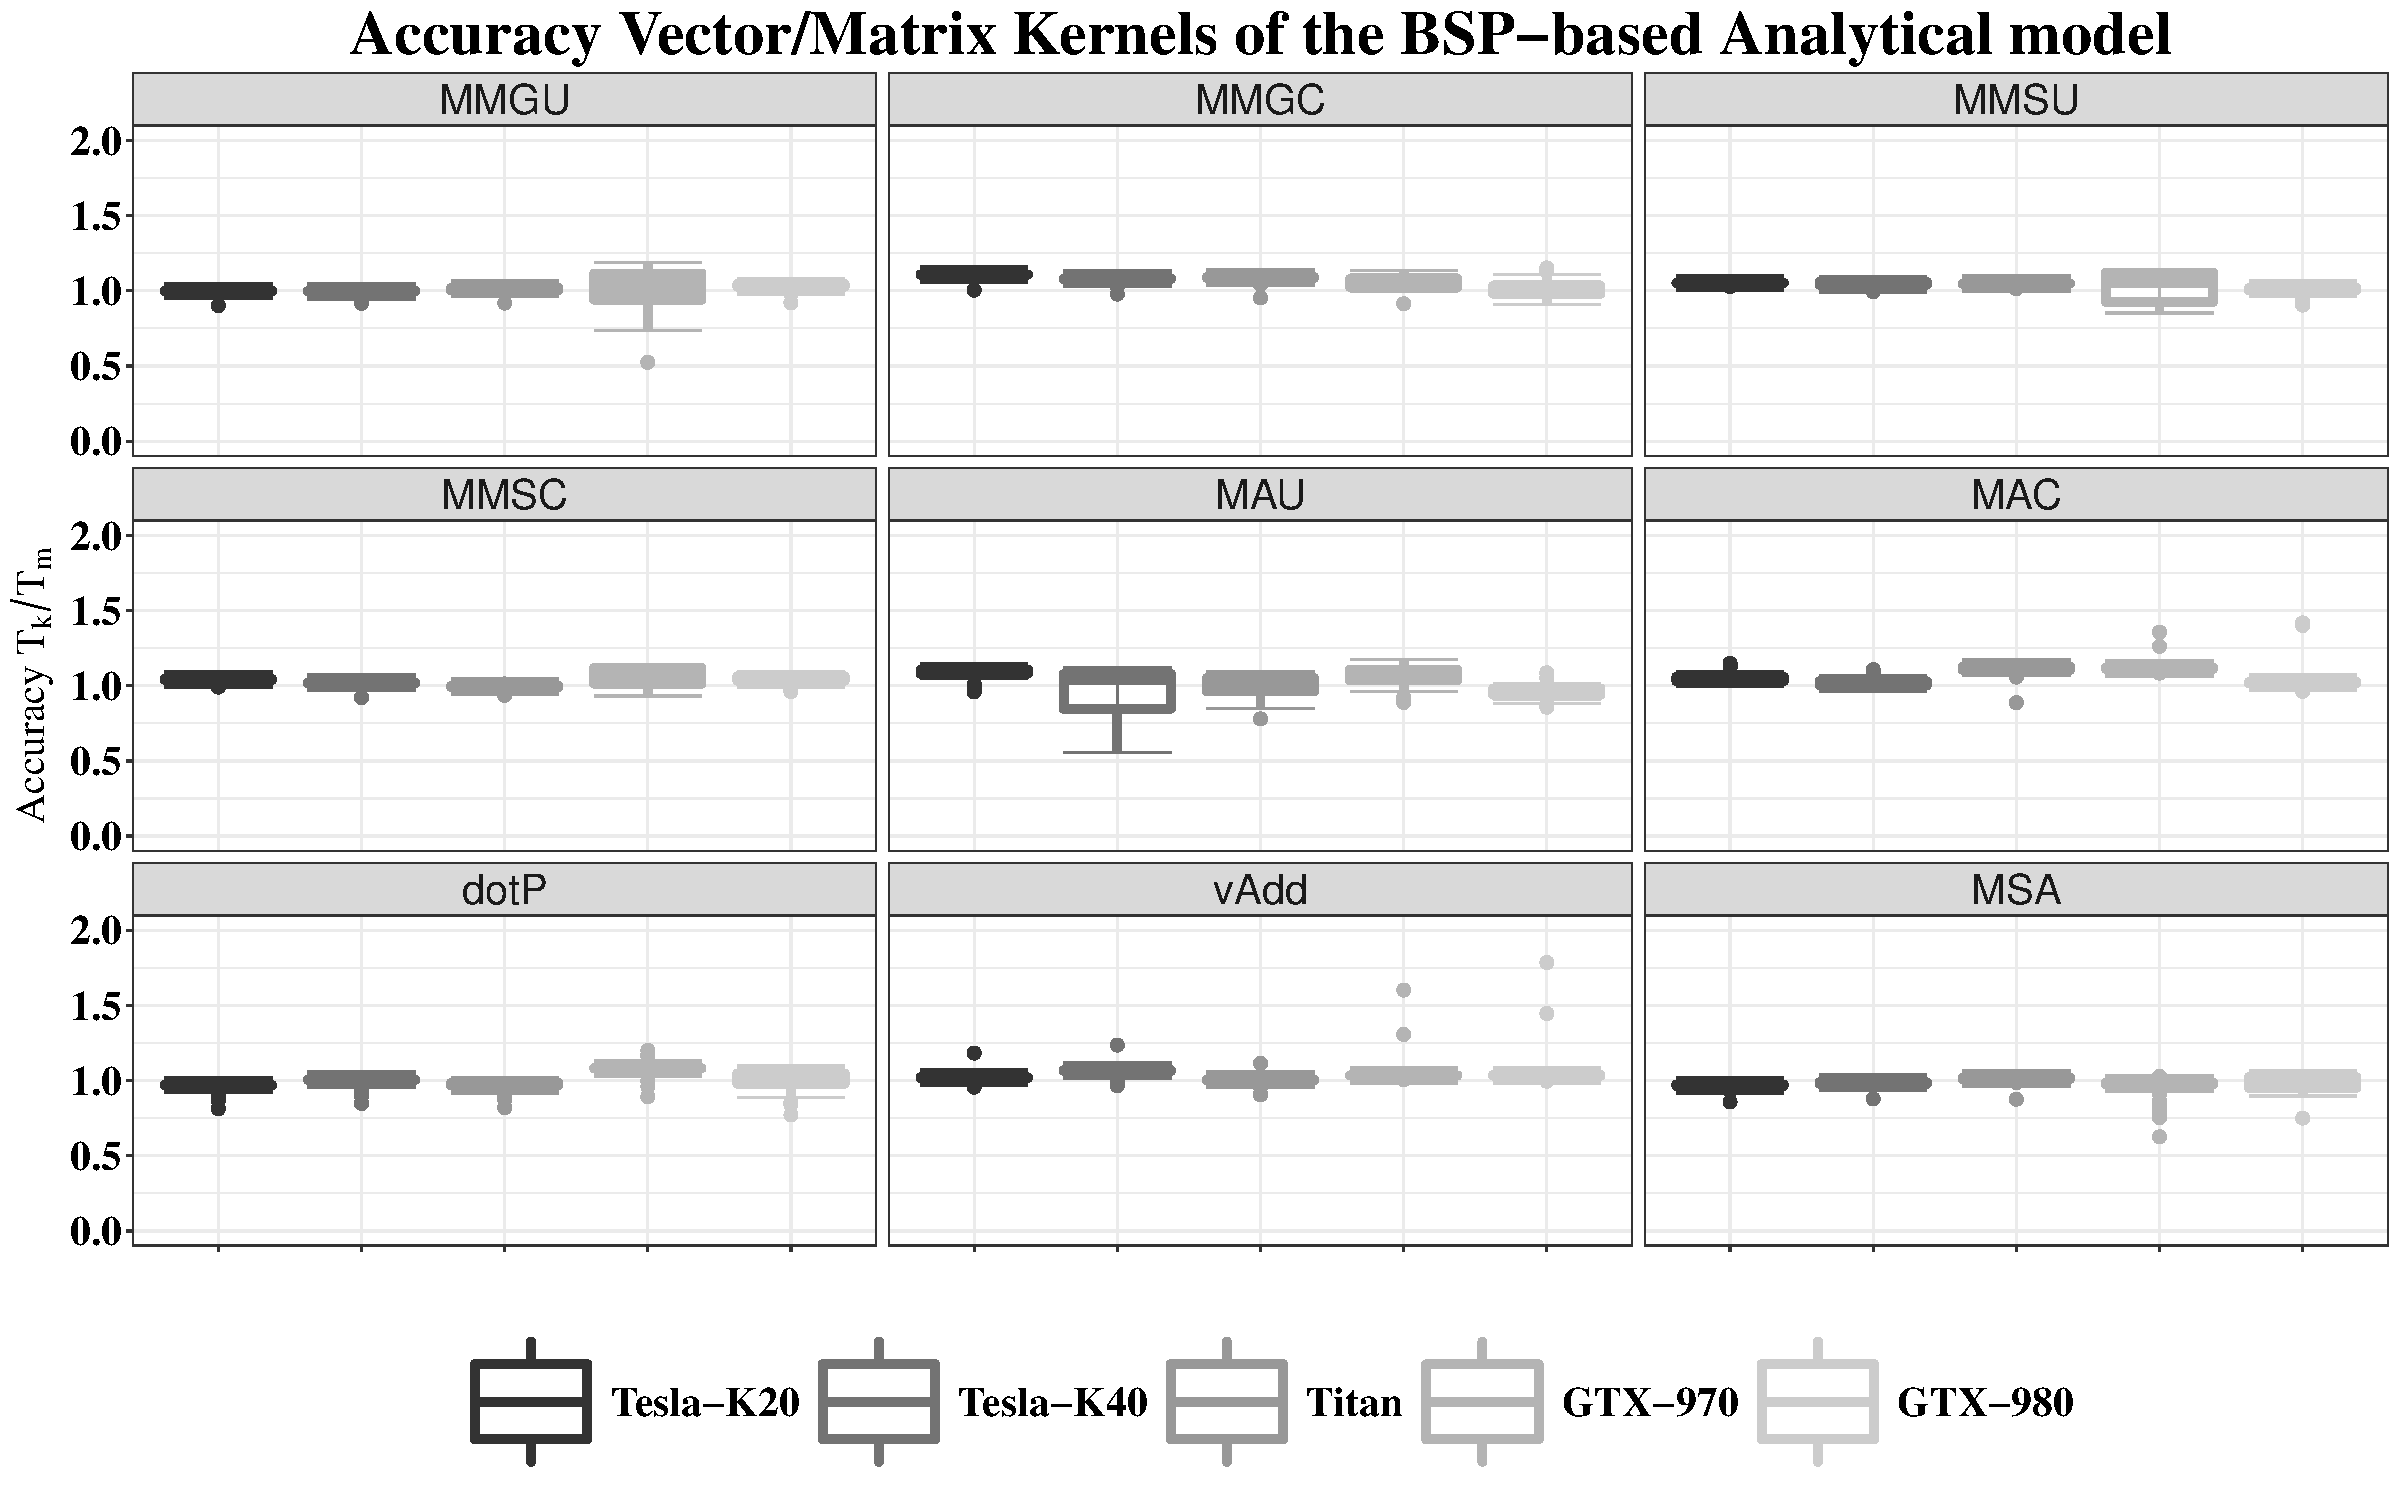
\includegraphics[scale=.4]{./images/ResutAnalyticalModel.pdf}
\caption{$T_k/T_m$  of vector and matrix algorithms with different values of $\lambda$, see table~\ref{tab:Lambda-NCA}}
\label{fig:resultsVMApp}
\end{figure}


Figure~\ref{fig:ResultsRodinia} shows the rate between the predicted and measured times of each one of the selected Rodinia CUDa kernels for the all the GPUs. This figure shows that predictions of the kernels BCK-1, BCK-2, HTW and HOT were between 0.9 and 1.1, showing a good prediction capability of the model. It was not possible to predict correctly the execution times of the kernels (GAU-1) and (GAU-2) because in both kernels the number of threads decrease in a loop during the execution of whole application. In both kernels execution around 10 threads are launched. GAU-K1 and GAU-K2 in each iteration of their execution decrease the number of threads and consequently the number of instructions. These instruction variations degraded the throughput significantly and the model required calibration of the parameter $\lambda$ or another adjustable parameter. These samples of GAU-K1 and GAU-K2 represented in big outliers and we have decided solve it in a future, adding parameters based on throughput. 

\begin{figure}[htpb]
\centering
 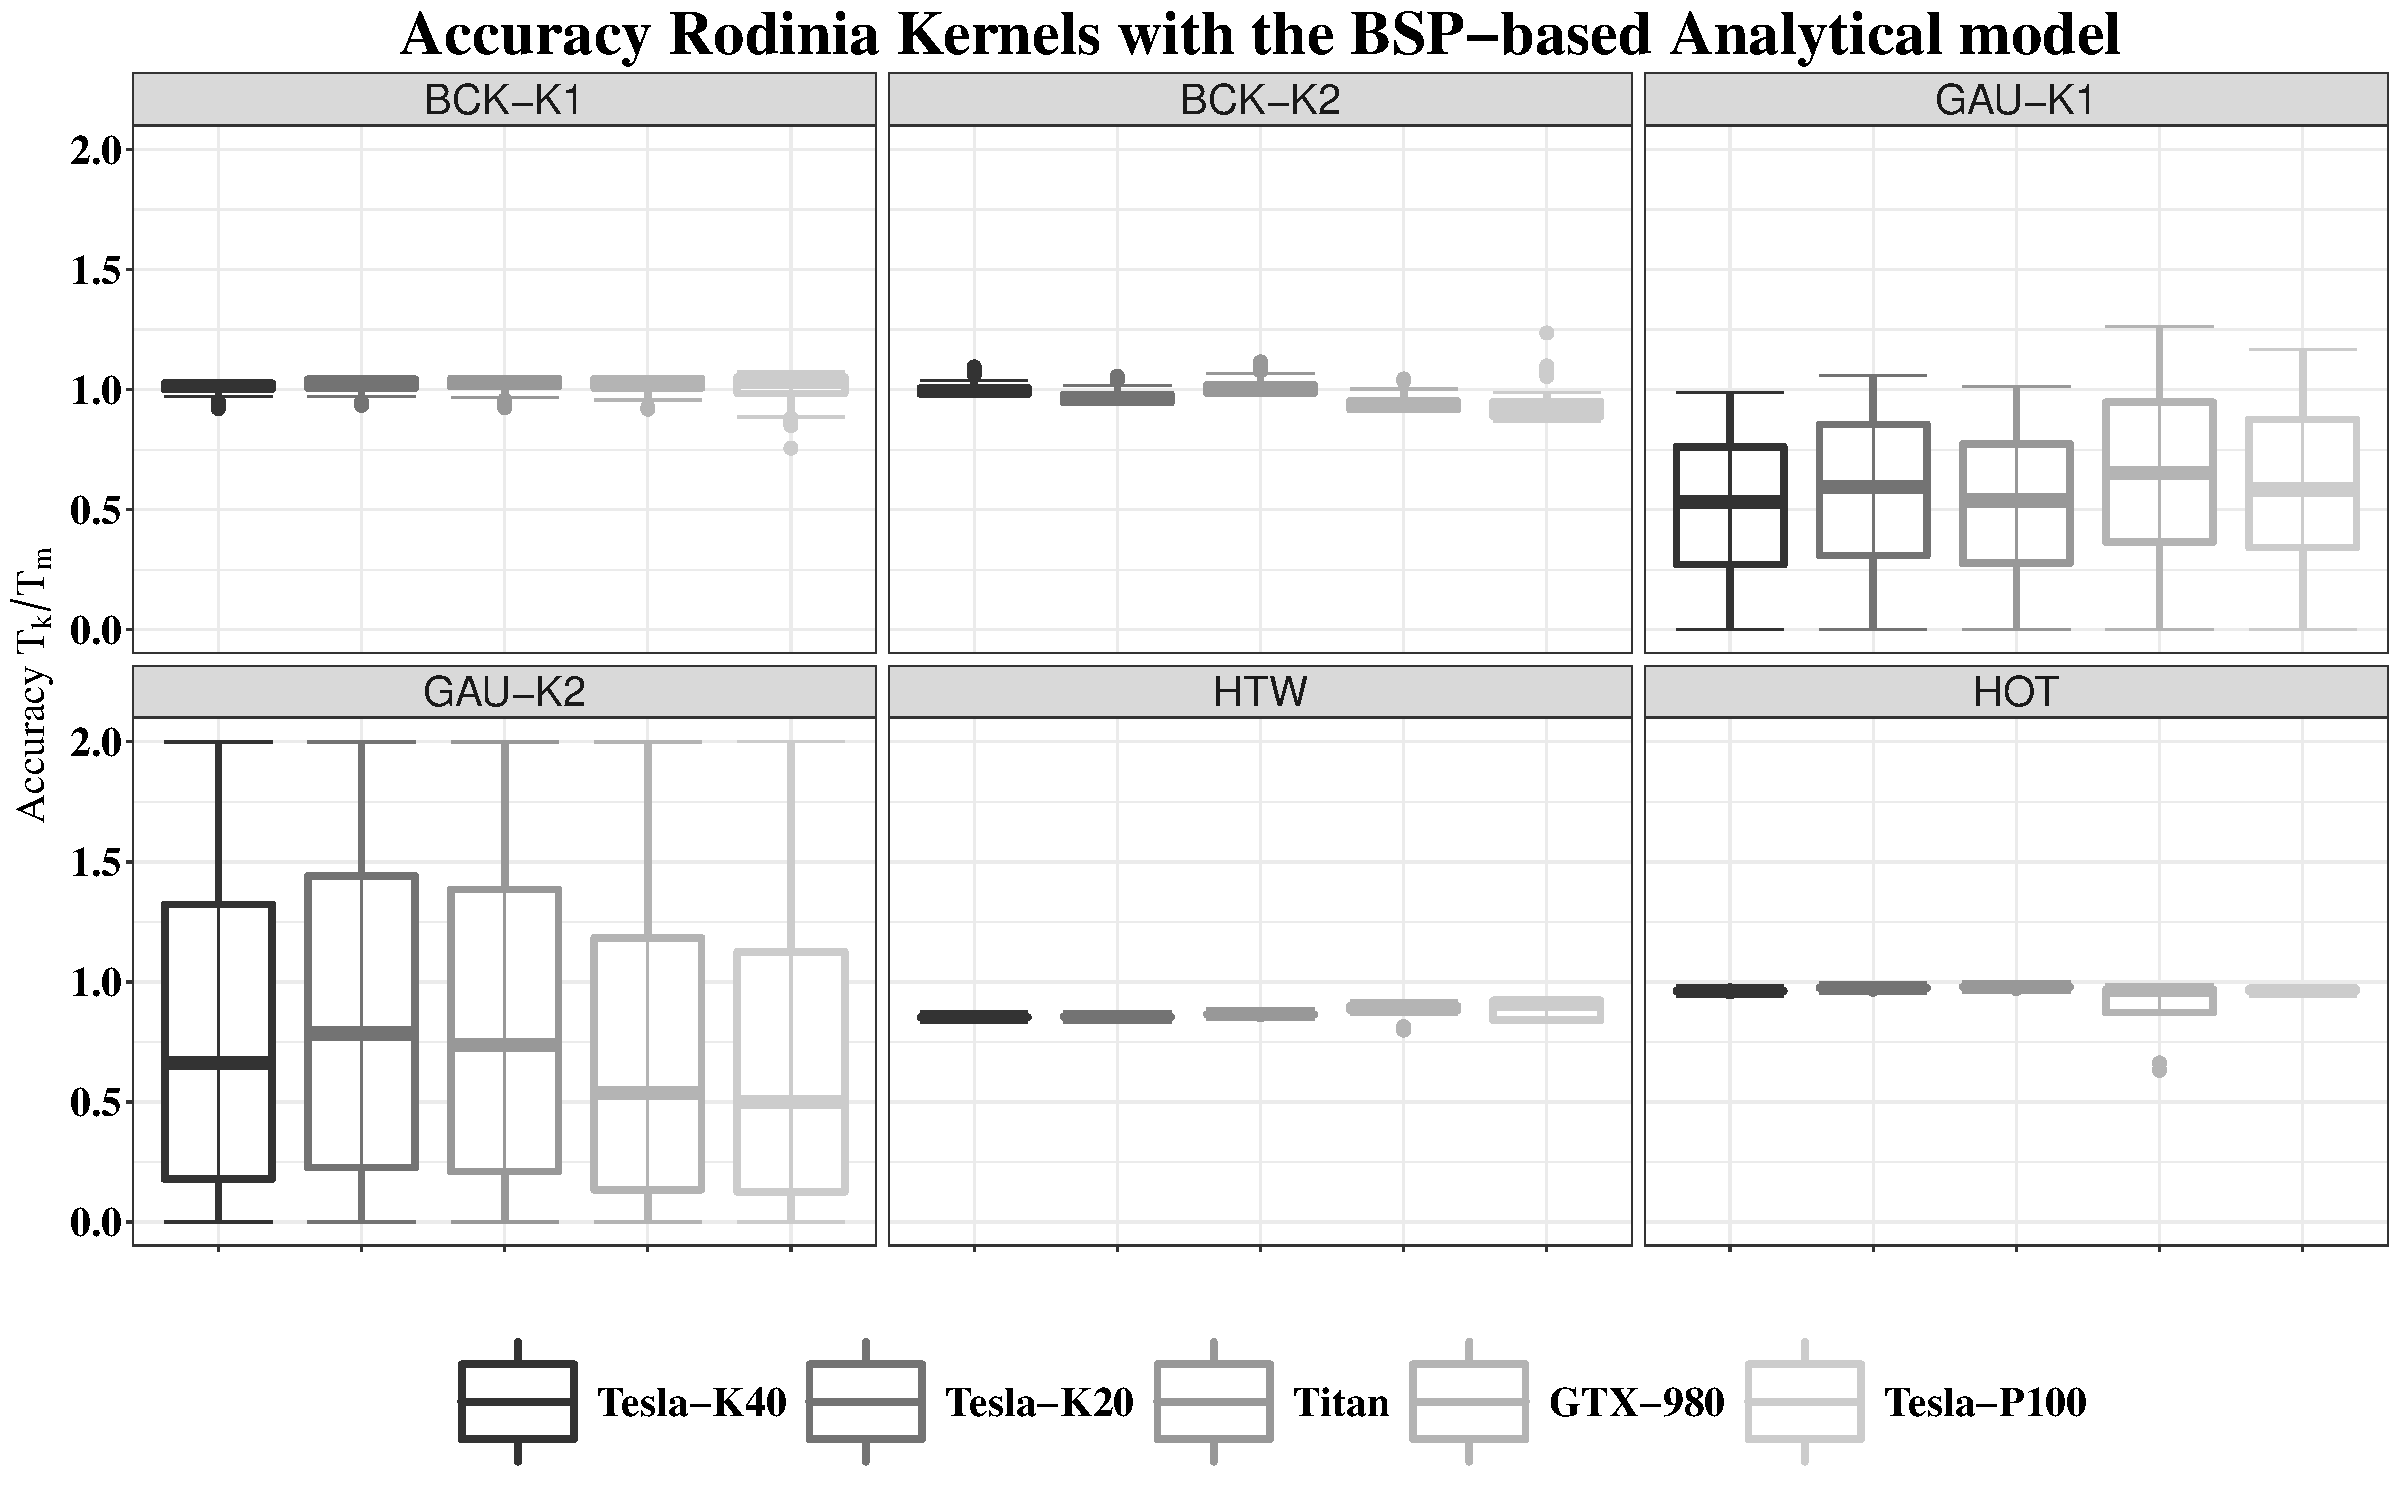
\includegraphics[scale=.4]{images/ResutAnalyticalModelRodinia.pdf}
\caption{$T_k/T_m$  of Rodinia CUDA kernels with different values of $\lambda$, see table~\ref{tab:lambdaRodinia}}
\label{fig:ResultsRodinia}
\end{figure}


These results show that we can use the model in the scenarios with different GPU types of the same architecture and with only one GPU type. In both cases the model can predict applications execution time from measurements on a single board with a single input size. With different GPU types, the prediction is less precise, since the optimal $\lambda$ value is different for each board. But it can still produce adequate predictions.

By considering two levels of memory, shared and global memories, we could accurately model the performance of these applications using several GPU models and problem sizes. The usage of two adaptable parameters $\lambda$ was sufficient to model the effect of data coalescing during read and write operations to the global memory. A similar set of parameters also model the effects of cache hits, computation and communication process of any GPU application. In the majority of the scenarios, the time measured were around $0.8$ to $1.2$ times the model predicted execution time. 

Next section will present some main related works using analytical model to predict GPU applications.

\section{Related Works}\label{sec:relatedModel}
To ease the development and analysis of parallel programs, the BSP programming model has been implemented as API libraries~\citep{BSPLib}, and recently enhanced to simplify programming on GPU architectures~\citep{bsgp}. These developments help to create scientific applications in massively parallel environments computing in an easier and better way.

In  recent  years,  studies on GPU performance using analytical modeling have appeared, most of them have also used NVIDIA cards in their experiments. \cite{GpuModelHong:2009} have proposed and evaluated a memory and parallelism-aware analytic model to estimate execution time of massively parallel application in GPUs. The key idea is to find a metric which they have called MWP (Memory Warp Parallelism) and CWP (Compute Warp Parallelism). The analytic model provides good performance predictions, however, this model requires a deep analysis and understanding by third-party developers of parallel applications in CUDA. They have introduced the metrics MWP and CWP, MWP is related to how much memory parallelism in the application and CWP is related to the program characteristics. CWP is used to decide whether performance is dominated by computation or communication. 

~\cite{PredicModelGPU2009} have presented a combination of known models with small extensions. The models they have used are: BSP model, PRAM model by~\citep{Fortune:1978:PRAM} and the QRQW model by~\cite{Gibbons1983:QRQW}. The authors abstract the GPU computational model by considering the pipeline characteristic of the application in GPU architectures. But they do not describe how divergence can impact in the efficiency of GPU applications. 

~\cite{Zhang:2011:GPUmodel} have presented a quantitative performance analysis model, based on micro-benchmarks for NVIDIA GeForce 200-series GPUs. They have developed a throughput model for three components of GPU execution time: the instruction pipeline, shared memory access, and global memory access. The model is based on a native GPU instruction set instead of the intermediate PTX assembly language or a high-level language. Our model uses a high-level bridging model for parallel computation and is focused on computation and communication processes for any GPU application. This encourage developers to use better optimizations in communication and computation.

~\cite{Kerr:2012:Eiger} developed a methodology for the systematic construction of performance models of heterogeneous processors. This methodology is comprised of experimental data acquisition and database construction, a series of data analysis passes over the database, and model selection and construction. They developed a framework, named Eiger, that implements their methodology. Another framework to construct performance models was presented by~\cite{Spafford:2012:Aspen}. They used a domain specific language to develop analytical performance models for the three dimensional Fast Fourier Transform (3D FFT).  

Our model is based solely in the BSP model. Scalability, optimization effects, divergence and differences between architectures are all adjusted by a single parameter $\lambda$. Profiling techniques were used to confirm information about caches memories accesses and to establish parameters about computation and communication when this parameters were difficult to find in the source code of the kernels. This model allows an easy parametrization, well-suited for many CUDA kernels in productions.
\todoMT{Compare between both related works sections}

